\chapter{Iteración 3}

\begin{quotation}[Polymath]{Leonardo da Vinci (1452--1519)}
Simplicity is the ultimate sophistication.
\end{quotation}

\begin{abstract}
Esta iteración amplía la estructura del juego con sistemas que refuerzan la identidad de
la experiencia. Se desarrolla una lógica de contenidos por círculo, se incorpora la
dualidad de personajes y se introduce una primera versión del minimapa como apoyo a la
navegación.
\end{abstract}

\section{Análisis de características}
La tercera iteración se dedicó a ampliar el núcleo del sistema y a reforzar la integración
entre progresión, personaje e interfaz. Una vez establecida en la iteración anterior la
base del descenso entre círculos, el siguiente paso lógico consistía en hacer que cada
círculo no fuera solo un número o una etiqueta en pantalla, sino una unidad real de
contenido con impacto sobre las salas y enemigos que aparecen en la partida. Al mismo
tiempo, también resultaba necesario introducir la primera versión jugable de la dualidad de
personajes y ofrecer al jugador una ayuda visual mínima para orientarse dentro de los mapas
generados.

Por ello, esta iteración se articula alrededor de tres funcionalidades: la consolidación de
la lógica de círculos como sistema de contenido, la incorporación de la dualidad de
personajes y la implementación inicial del minimapa.

\begin{enumerate}
\item \textbf{Lógica de círculos.} En esta iteración la lógica de círculos dejó de actuar
únicamente como mecanismo de progresión secuencial y pasó a convertirse en el sistema que
organiza el contenido del juego por niveles temáticos. Su funcionamiento real consistió en
asociar a cada círculo una definición propia con nombre, conjunto de salas disponibles y
pool ponderado de enemigos, de forma que al descender no solo cambie el valor del círculo
actual, sino también el contenido que el generador y el gestor de habitaciones emplean para
construir la siguiente partida. Esto permitió que la progresión dejara de ser puramente
abstracta y comenzara a reflejarse en el mundo jugable. Además, la feature introdujo una
base escalable para trabajar con nueve círculos diferenciados sin endurecer la lógica del
sistema en código fijo, desplazando la configuración a estructuras de datos reutilizables.
En términos funcionales, esto significa que el juego ya no genera un único conjunto de
salas y enemigos para todas las partidas, sino que adapta su contenido al círculo en el que
se encuentra el jugador.

\begin{figure}[H]
\begin{center}
\missingfigure{Sustituir por captura representativa de Lógica de círculos en la iteración 3}
% \includegraphics[width=.9\textwidth]{figures/iteracion3_logica_circulos.png}
\caption{Resultado visual de la feature Lógica de círculos en la iteración 3}
\label{fig:iteracion3-feature-circulos}
\end{center}
\end{figure}

\item \textbf{Dualidad de personajes.} Esta funcionalidad introdujo la primera versión
realmente jugable del sistema de dualidad, modelándolo como un cambio entre dos formas de
combate complementarias: una forma cuerpo a cuerpo y una forma a distancia. Su
comportamiento real no consistía en duplicar personajes independientes, sino en permitir
que el mismo jugador alterne entre dos estados con identidad visual propia, manteniendo
estadísticas compartidas y sujeto a un tiempo de reutilización para evitar cambios
instantáneos sin coste. La feature integra, por tanto, tres piezas: la representación de la
forma actual, la lógica de intercambio con \textit{cooldown} y la persistencia del estado
compartido entre ambas variantes. Con ello se consigue que la dualidad deje de ser una idea
de diseño y pase a actuar como una mecánica concreta de juego sobre la que podrán apoyarse
futuras habilidades, sistemas de combate y decisiones tácticas.

\begin{figure}[H]
\begin{center}
\missingfigure{Sustituir por captura representativa de Dualidad de personajes en la iteración 3}
% \includegraphics[width=.9\textwidth]{figures/iteracion3_dualidad_personajes.png}
\caption{Resultado visual de la feature Dualidad de personajes en la iteración 3}
\label{fig:iteracion3-feature-dualidad}
\end{center}
\end{figure}

\item \textbf{Minimap.} Esta funcionalidad incorporó una primera versión muy simple del
minimapa orientada a cubrir una necesidad básica de orientación. Su funcionamiento real se
apoya en la propia estructura de celdas generadas por el mapa, reutilizando esa
representación para mostrar qué salas han sido descubiertas y cuáles permanecen ocultas
todavía. La feature no pretende en esta iteración ofrecer una interfaz sofisticada, sino
dar una lectura mínima del avance del jugador por la mazmorra. Para ello se introdujo un
sistema de descubrimiento progresivo: la sala inicial aparece visible desde el comienzo y,
a medida que el jugador entra por primera vez en nuevas habitaciones, estas pasan a marcarse
como descubiertas. Esta solución refuerza la legibilidad de la exploración sin añadir una
gran complejidad técnica y sirve como base para versiones más completas del minimapa en
iteraciones posteriores.

\begin{figure}[H]
\begin{center}
\missingfigure{Sustituir por captura representativa de Minimap en la iteración 3}
% \includegraphics[width=.9\textwidth]{figures/iteracion3_minimap.png}
\caption{Resultado visual de la feature Minimap en la iteración 3}
\label{fig:iteracion3-feature-minimap}
\end{center}
\end{figure}
\end{enumerate}

La combinación de estas tres funcionalidades hizo que la tercera iteración ya no estuviera
centrada solo en estabilizar la base del juego, sino en empezar a dotarla de identidad
propia. La progresión por círculos adquirió contenido real, el jugador ganó una mecánica
diferenciadora y la exploración recibió un primer apoyo visual permanente.

\section{Diseño}
El diseño de esta iteración se construyó sobre una idea común: desplazar decisiones
específicas desde lógica rígida hacia estructuras capaces de evolucionar con el proyecto.
En vez de seguir ampliando el prototipo mediante soluciones puntuales, se buscó dejar
preparados mecanismos más generales para que el sistema pudiera crecer con nuevas variantes
de contenido y con nuevas capas de interacción.

\subsection{Diseño de la lógica de círculos como sistema de contenido}
La principal decisión de diseño consistió en transformar los círculos en unidades de
configuración de contenido. En lugar de utilizar una única colección global de salas y
enemigos para todo el juego, se diseñó una base de datos de círculos que permite definir,
para cada uno de ellos, su nombre visible, su pool de habitaciones y su pool ponderado de
enemigos.

Este enfoque tiene dos ventajas relevantes. La primera es que desacopla la progresión del
contenido concreto, permitiendo que el sistema consulte la definición del círculo actual en
lugar de depender de una lógica distribuida por múltiples scripts. La segunda es que
facilita la escalabilidad, ya que añadir o ajustar círculos pasa a ser principalmente una
operación de configuración y no una reescritura del comportamiento interno del generador.

\subsection{Diseño de la dualidad de personajes}
La dualidad se diseñó como una alternancia de formas y no como una sustitución de entidades
completamente independientes. Esta decisión resultaba más coherente con el estado del
proyecto, porque permitía introducir la mecánica sin duplicar toda la lógica del jugador ni
forzar todavía un sistema complejo de persistencia externa.

Sobre esa base se definieron dos principios. El primero, que ambas formas debían compartir
el estado fundamental del personaje, especialmente la salud, los recursos y la capacidad
básica de movimiento. El segundo, que el intercambio debía tener una restricción temporal,
de modo que el cambio no se convierta en una acción sin coste ni ritmo. También se decidió
dar a cada forma una representación visual diferenciada para que el cambio fuera legible de
inmediato dentro de la partida.

\subsection{Diseño del minimapa}
El minimapa se planteó como una proyección simplificada del propio modelo del nivel. La
decisión importante aquí fue no construir una representación completamente independiente,
sino reutilizar las celdas ya generadas por el sistema como soporte del mapa visual.

Además, se optó por un modelo de niebla de descubrimiento muy simple: las salas no
descubiertas se mantienen con opacidad nula o reducida, mientras que las visitadas pasan a
mostrarse plenamente. Este diseño encaja bien con la fase del proyecto, porque aporta valor
jugable inmediato sin exigir todavía una gran complejidad en iconografía, navegación o
interacción.

\section{Implementación}
La implementación de esta iteración combinó incorporación de nuevos objetos de
configuración, ampliación de lógica de jugador y ajustes sobre el generador del mapa. A
diferencia de la segunda iteración, donde predominaban los mecanismos de transición y
estabilidad, aquí el peso recae más en la organización del contenido y en la introducción
de nuevas capas de comportamiento jugable.

\subsection{Implementación de la lógica de círculos}
La feature se materializó mediante dos nuevos tipos de \textit{Scriptable Objects}:
\texttt{CircleDefinition}, que encapsula la configuración de un círculo concreto, y
\texttt{CircleDatabase}, que centraliza el acceso a todas las definiciones disponibles. A
partir de ahí, el \texttt{CircleManager} se amplió para mantener no solo el número de
círculo actual, sino también una referencia a la definición activa correspondiente.

Esta ampliación tuvo consecuencias directas sobre el resto del sistema. El
\texttt{RoomManager} dejó de depender exclusivamente de un pool global de habitaciones y
pasó a consultar el pool específico del círculo actual para decidir qué sala instanciar en
cada caso. Del mismo modo, la selección de enemigos pasó a realizarse a partir de entradas
ponderadas asociadas al círculo, permitiendo filtrar por tipo de habitación y variar el
contenido según el contexto.

En la práctica, la implementación convirtió el descenso entre círculos en un cambio real de
configuración del mundo: al actualizarse el círculo activo, cambia también el conjunto de
salas y enemigos que el sistema utiliza para construir la nueva planta.

\subsection{Implementación de la dualidad de personajes}
La dualidad se implementó principalmente en el script \texttt{Player}. Se introdujo una
enumeración para distinguir entre forma de melé y forma a distancia, una configuración de
forma inicial, un tiempo de reutilización para el intercambio y referencias visuales
independientes para cada estado.

La lógica de cambio se articula en torno a una acción específica de entrada que solicita el
intercambio, comprueba si el \textit{cooldown} ha expirado y, si procede, activa la forma
contraria. Paralelamente, el jugador mantiene estadísticas compartidas, como salud,
recurso máximo y daño base, de modo que el cambio de forma altera la representación y el
estado táctico, pero no rompe la continuidad del personaje.

También se añadió un evento de cambio de forma, lo que deja preparada la posibilidad de que
otros sistemas reaccionen a la dualidad en iteraciones posteriores. Aunque en esta fase la
feature todavía no explota todas sus implicaciones de combate, la implementación deja ya
resuelto el esqueleto funcional del sistema.

\subsection{Implementación del minimapa}
La primera versión del minimapa se integró directamente en \texttt{MapGenerator}. Se añadió
un conjunto de índices de salas descubiertas y una lógica de inicialización que marca como
visible la habitación inicial al comenzar una nueva partida. A partir de ahí, cada vez que
el jugador entra por primera vez en una sala, el sistema registra sus celdas y actualiza la
apariencia del mapa.

La actualización visual se resuelve modificando la opacidad de los elementos que representan
cada celda, distinguiendo entre habitaciones descubiertas y no descubiertas. También se
añadieron ajustes en el prefab de celda para facilitar esta visualización y un controlador
de interfaz mínimo asociado al HUD del minimapa. Aunque esta versión todavía es sencilla,
la implementación logra el objetivo principal de la feature: ofrecer una lectura progresiva
del recorrido del jugador por el nivel generado.

\section{Seguimiento y control}
El seguimiento de esta iteración confirmó que el alcance principal podía cumplirse, aunque no
todas las funcionalidades alcanzaron el mismo grado de madurez. La lógica de círculos sí
quedó consolidada en el sentido previsto, porque dejó de ser una mera progresión numérica y
pasó a organizar contenido real del juego. De forma similar, la dualidad de personajes quedó
cerrada como primera versión jugable y suficientemente estable para apoyar iteraciones
posteriores.

Desde el punto de vista temporal, la iteración registró una ligera desviación respecto a la
planificación: frente a las 50:00 horas previstas, se emplearon 51:41 horas reales. La
diferencia es pequeña, pero el seguimiento del trabajo sí puso de manifiesto que el minimapa
no convenía darse por terminado en esta fase si se quería mantener un cierre coherente del
alcance.

La primera versión del minimapa cumplía su función básica de orientación, pero aún dependía
de ajustes posteriores sobre el estado real de las salas, la cámara y su integración en el
HUD. Por ello, se optó por cerrar en esta iteración una versión funcional mínima y
replanificar su segunda parte para la iteración 6, cuando el resto de sistemas implicados ya
estuviera más estabilizado. Esta decisión permitió ajustar el alcance a la complejidad real
sin perder el control de la planificación general.

\begin{table}[h!]
    \centering
    \begin{coolTable}{lr}{2}
    {Horas de la iteración 3}
    \textbf{Horas planificadas de la iteración} & 50:00 \\
    \textbf{Horas reales (Adolfo Borrego González)} & 28:15 \\
    \textbf{Horas reales (Germán Sánchez Carmona)} & 23:26 \\
    \textbf{Horas reales totales de la iteración} & 51:41 \\
    \textbf{Horas acumuladas planificadas hasta esta iteración} & 250:00 \\
    \textbf{Horas acumuladas reales hasta esta iteración} & 247:54 \\
    \end{coolTable}
    \caption{Resumen de horas reales de la iteración 3.}
\end{table}

\begin{figure}[htbp]
\begin{center}
% \missingfigure{Sustituir por el diagrama UML de resultado de la iteración 3}
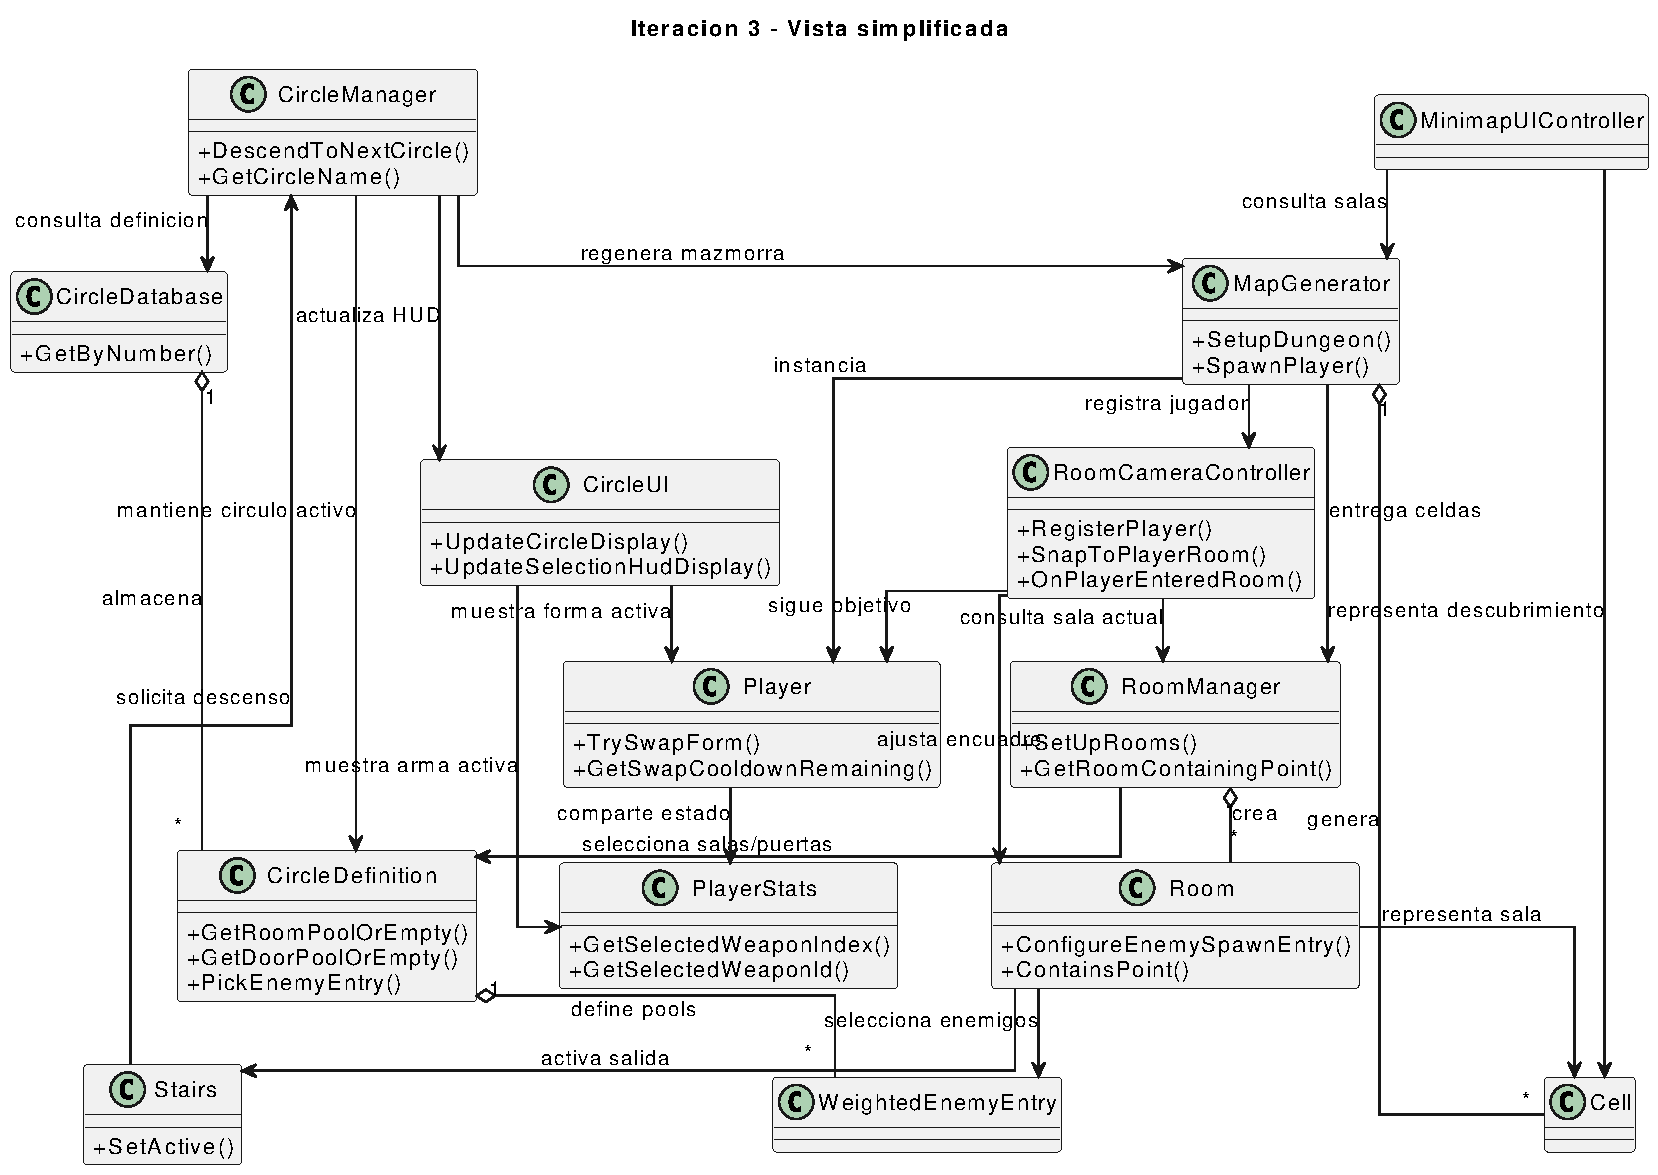
\includegraphics[width=\textwidth]{figures/iteracion3_resultado_uml.pdf}
\caption{Diagrama UML de resultado de la iteración 3}
\label{fig:uml-resultado-iteracion3}
\end{center}
\end{figure}
